\chapter{ORB-SLAM at the edge} \label{chap:verification}
This chapter will focus on description, verification and customization of ORB-SLAM2 \cite{murORB2} for execution on a low-power heterogeneous embedded device (i.e. NVIDIA Jetson TX2). Primary it will describe how ORB-SLAM2 works. Secondly it will show an accurate inspection necessary to find some potential bugs that cause an unexpected behaviour of the algorithm.

 \section{System description}
 As described in \cite{iros2019}, ORB-SLAM2 is a Simultaneous Localization And Mapping system that can works with data coming from monocular, stereo, and RGB-D cameras. A system of this kind has the purpose to allow both map reconstruction and navigation in the most common environment without the support of a GPS.
 The system consists of the following three main blocks (see figure \ref{fig:orbslam}):

\begin{description}
	\item[Tracking and localization] 
	This block is in charge of computing visual features, localizing the robot in the environment, and, in case of significant discrepancies between an already saved map and the input stream, communicating updated map information to the mapping block. The frames per second (FPS) that can be computed by the whole system strongly depends on the performance of this block.
	\item[Mapping] 
	It updates the environment map by using the information (map changes) sent by the localization block. It is a computational time consuming block and its execution rate strictly depends on the agent speed. However, considering the actual agent speed of the KITTI datasets analysed in this work \cite{CVPR2012}, it does not represent a system bottleneck.
	\item[Loop closing] 
	It aims at adjusting the scale drift error accumulated during the input analysis. When a loop in the robot pathway is detected, this block updates the mapped information through a high latency heavy computation, during which the first two blocks are suspended. This can lead the robot to loose tracking and localization information and, as a consequence, the robot to get temporary lost. The computation efficiency of this block (running on-demand) is crucial for the quality of the final results.
\end{description}

\begin{figure}
	\centering
	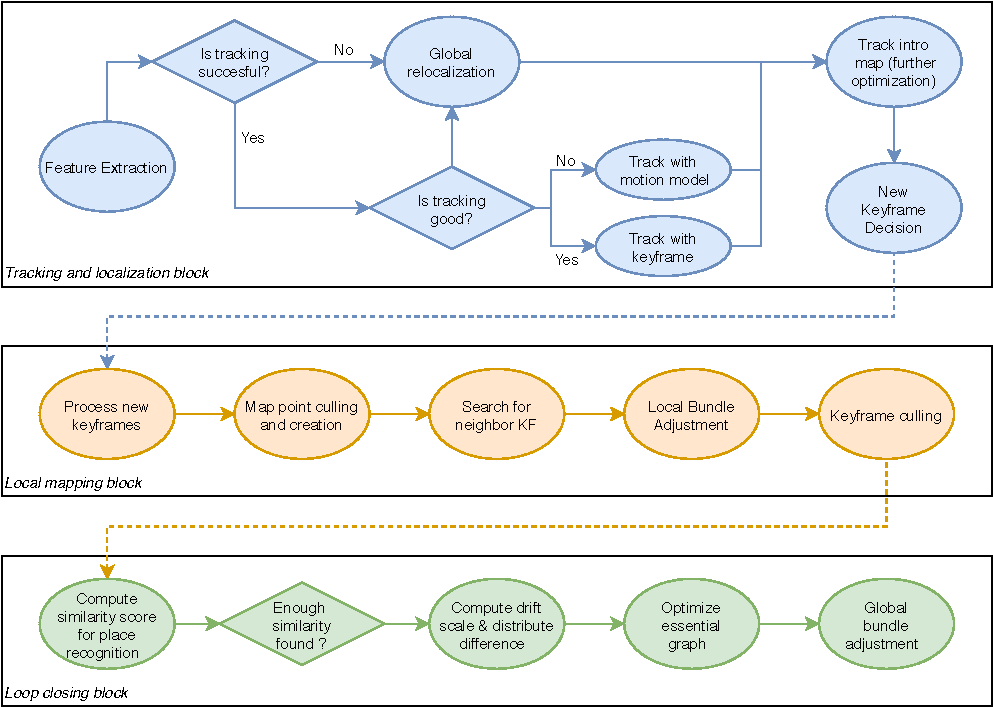
\includegraphics[width=0.90\textwidth]{images/orb-slam-overview2.pdf}
	\caption{Main blocks of the ORB-SLAM2 algorithm.}
	\label{fig:orbslam}
\end{figure}


The system is organized on three parallel threads, one per block. The use of parallel threads allows for obtaining real-time processing on an Intel Core i7 desktop PC with 16GB RAM \cite{murORB2}. The original open source version of ORB-SLAM2 provides two level of parallelism. The first level is given by the three main algorithm blocks (see Fig. \ref{fig:orbslam}), which are implemented to be run as parallel PThreads on shared-memory multi-core CPUs. The second level is given by the automatic parallel implementation (i.e., through OpenMP directives) of the \textit{bundle adjustment} sub-block, which is part both of the local mapping and loop closing blocks. This allows the parallel computation of such a long latency task on multi-core CPUs.
To fully exploit the heterogeneous nature of the target NVIDIA Jetson TX2 board, the work done in \cite{iros2019} added two further levels of parallelism. The first is given by the parallel implementation for GPU of a set of tracking sub-blocks (see Fig. \ref{FIG:FE-DAG}). This is because the most important bottleneck that characterizes the processing rate in terms of supported FPS, was detected on the feature extraction block. The second is given by the implementation of a 8-stage pipeline of such sub-blocks in order to benefit of an overlapped computation.

\begin{figure}[t!]
	\centering
	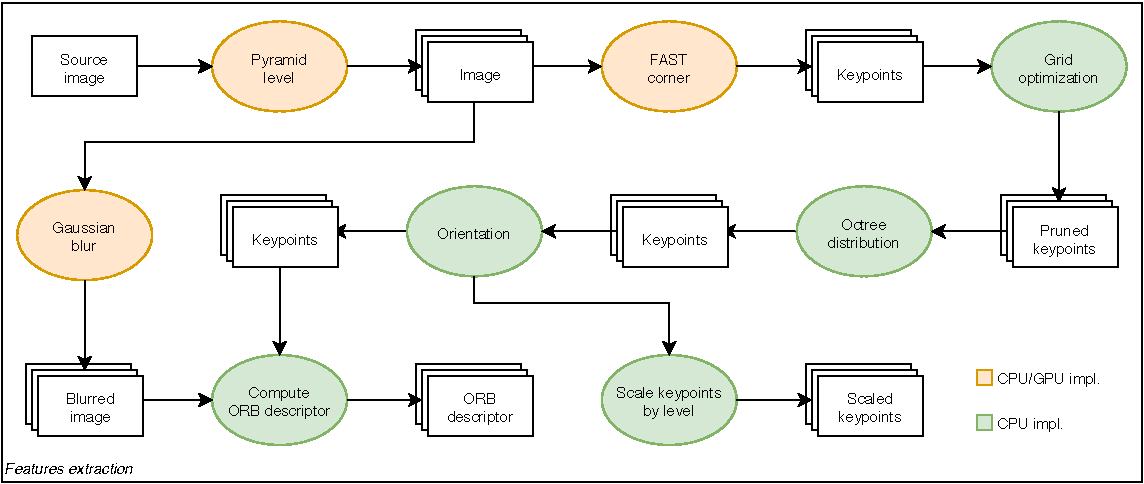
\includegraphics[width=\linewidth]{images/orb-feature.pdf}
	\caption{DAG of the feature extraction block and the corresponding sub-block implementations (GPU vs. CPU).}\label{FIG:FE-DAG}
\end{figure}


%TODO pensavo qui di riportare un riassunto della sezione A della metodolgia del paper di IROS ed un paio di risultati sperimentali ...


%%%%%%%%%%%%%%%%%%%%%%%%%%%%%%%%%%%%%%%%%%%%%%%%%%%%%%%%%%%%%%%%%%%%%%%%%%
\section{Unexpected behaviour}
After the porting and the optimizations of the ORB-SLAM2 algorithm on the NVIDIA Jetson TX2 to achieve real-time performance, the experimental results conducted in \cite{iros2019} shown a massive improvement of the execution times on some KITTI dataset sequences.
Despite these performance improvements, the algorithm seems to exhibit some unexpected behaviours too frequently, especially with sequences that contain a higher space-temporal variation between one frame and the next one. After processing a frame the algorithm can be in three state: \textit{Not Initialized}, \textit{Track}, \textit{Lost}. The problem is that it get into the Track Lost state (fig. \ref{fig:lost}) after the initialization in a totally random way. Another Track Lost state is reached when less then 5 Keyframes are computed and it loses its position (see fig: \ref{fig:lost-reset}).

\begin{figure}[t]
	\centering
	\subfloat[Track lost state]{\label{fig:lost}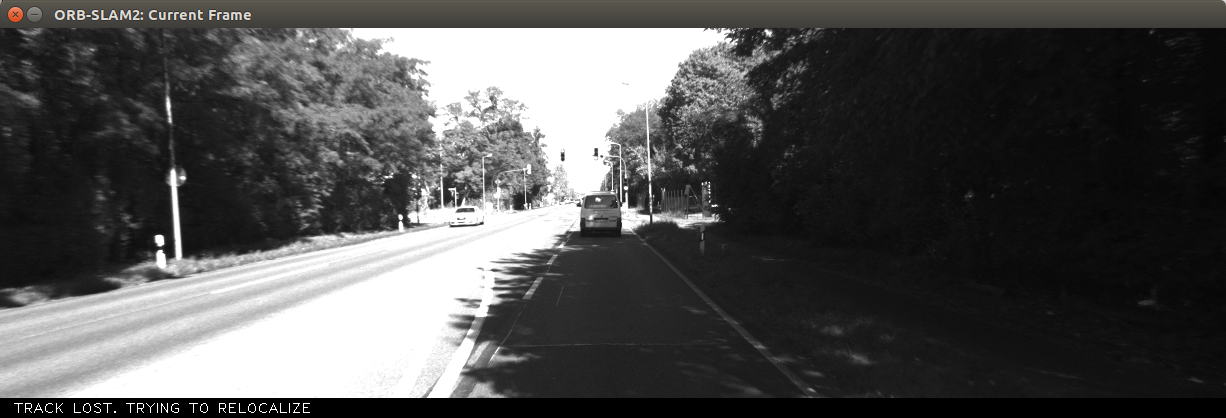
\includegraphics[width=0.9\linewidth]{images/track-lost-after-threshold}}
	\\
	\subfloat[Track lost soon after initialization, system resetting.]{\label{fig:lost-reset}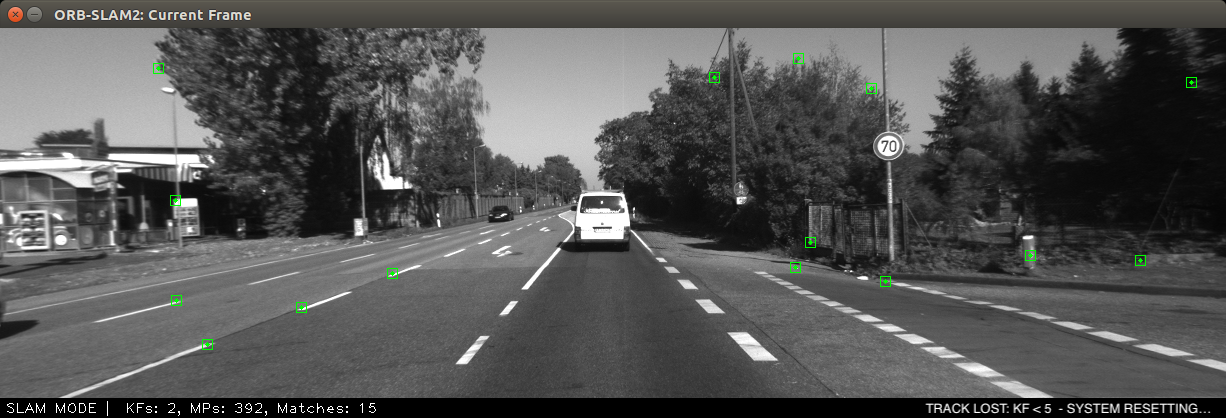
\includegraphics[width=0.9\linewidth]{images/Track-lost-soon-after-initialisation}}
	\caption{LOST states of ORB-SLAM2 in sequence 03 of KITTY dataset.}
\end{figure}

Due to the randomicity with which the problem occurs, to identify the cause it's necessary isolate the problem as much as possible. For this purpose the first step has been sequentialize the execution between Tracking and Mapping blocks.
Once the two blocks are running sequentially, we proceeded to inspect the code in more detail founding in such way some potential bugs.
The main strategy we adopted to find the possible problems within the code, was looking at the difference among the produced results after two o more sequential execution. To achieve this goal we built a custom logger with different levels of debugging.

An example of the problems we found is located in the KeyFrame source code, where a \mintinline{c++}{vector<pair<int, KeyFrame*>> vPairs} has been applied to the C++ standard \mintinline{c++}{sort} function. The problem here is the sort procedure use the less operator compare the address of the pointers instead of the id of the KeyFrame.
To solve this issue we override the less operator in order the achieve the expected behaviour (see listing \ref{lst:lessoverride}).
Another problem encountered during the code inspection that could introduce a non deterministic execution, is related to the members variables initialization.
Unlike some programming languages, C/C++ does not initialize most variables to a given value (such as zero) automatically. When a variable is assigned a memory location by the compiler, the default value of that variable is whatever (garbage) value happens to already be in that memory location! A variable that has not been given a known value (usually through initialization or assignment) is called an uninitialized variable.

\begin{listing}[tbp]
\begin{minted}[
fontsize=\footnotesize,
breaklines
]{C++}
namespace std {
    bool less<ORB_SLAM2::KeyFrame*>::operator()(
    const ORB_SLAM2::KeyFrame* k1,
    const ORB_SLAM2::KeyFrame* k2) const {
        return k1->mnId < k2->mnId;
    }
    bool operator<(const std::pair<int, ORB_SLAM2::KeyFrame*> lhs, const std::pair<int, ORB_SLAM2::KeyFrame*> rhs) {
        return lhs.first < rhs.first || ((lhs.first == rhs.first) && lhs.second->mnId < rhs.second->mnId);
    }
}
\end{minted} 
\caption{Overriding the less operator.}
\label{lst:lessoverride}
\end{listing}

Once these kind of problems have been resolved, the algorithm now is running with a deterministic behaviour. If it get into Track Lost state it happen every time and vice-versa. Unfortunately, when we restore the concurrency between Tracking and Mapping blocks, the problem of unexpected behaviour rise again.

To solve the problem we propose to revise in detail the implementation of the main algorithm for the localization. 
Finally it is also important note that the strategy adopted to achieve the goal can be applied in every application that runs in a concurrent and non-concurrent environment.


%\subsection{The problem of the non-determinism} % possible reasons that cause a non deterministic behaviour


%\subsection{The problem of the concurrency} % when we setup the orbslam to run sequentially it works worse that when it run concurrently.





\clearpage
\thispagestyle{empty}